\chapter{DoppelGANger : un générateur de séries temporelles puissant ... mais vulnérable}
    Ce chapitre s'appuie principalement sur l'article publié par l'équipe ayant développé le
    modèle DoppelGANger (\cite{doppelGANger}).
    \section{Particularités du modèle : comparaison avec un GAN classique}

        \subsection{Fonctionnement global}
            La principale contrainte reposant sur le GAN est la génération de séries
            temporelles. En effet l'architecture traditionnelle du GAN
            \textit{(MLP, Multi-Layer Perceptron)} n'est pas adaptée à la génération de telles
            données. L'architecture du DoppelGanger est donc une variante de RNN appelée LSTM (
            long-term short-term memory).

            Le fonctionnement du DoppelGanger, schématisé plus bas, est résumé comme suit par ses
            créateurs :

            \begin{enumerate}
                \item Capture des corrélations entre les métadonnées et les mesures, en
                utilisant un discriminateur auxiliaire
                \item Ajout de
                métadonnées factices capturant les valeurs minimales et maximales pour chaque
                échantillon généré pour remédier au problème d'effondrement des modes
                \footnote{production d'échantillons très similaires ou identiques, couvrant uniquement
                une partie limitée (un mode) de la distribution des données réelles, et ne représentant pas
                la diversité complète des données d'origine} concernant les mesures.
                \item Utilisation d'un générateur RNN par batchs
                pour capturer les corrélations temporelles et synthétiser de longues séries temporelles représentatives.
            \end{enumerate}

            \begin{figure}[H]
                \centering
                \fbox{
                    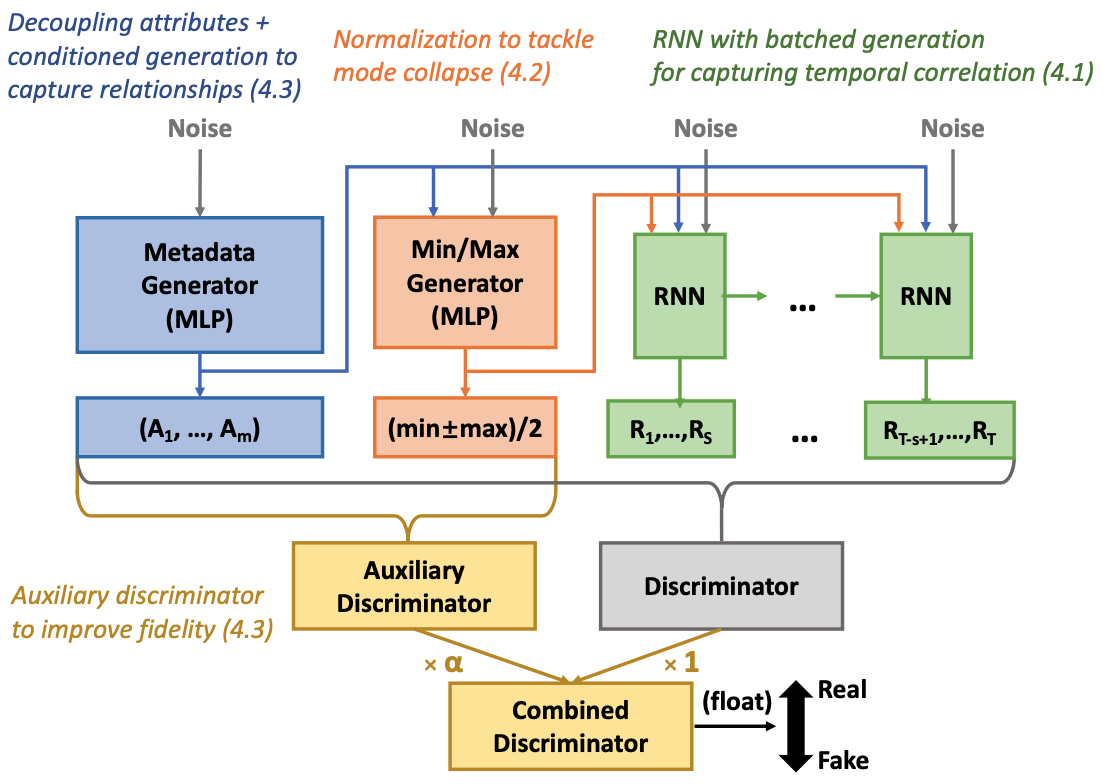
\includegraphics[width = 0.9
                    \textwidth]{figures/Resultats/ChapitreDopelGanger/dopelModel}}
                \caption{Architecture du DoppelGanger donnant les concepts clés et les extensions aux approches type Gan canoniques}
            \end{figure}
        \subsection{Hyperparamètres choisis pour la compétition}
            \begin{tcolorbox}[colback=linkborder_Color!5!white,colframe=linkborder_Color!75!black]
                Le modèle de la compétition n'inclut pas de métadonnées dans ses entrées et sorties, pour des raisons de simplicité.
            \end{tcolorbox}
                \begin{table}[H]
                    \centering
                    \begin{tabular}{p{0.5\textwidth}|p{0.35\textwidth}} \toprule
                        \textbf{Paramètre} & Valeur \\
                        \midrule
                            Taille du batch & $200$ \\
                            Taux d'apprentissage du générateur & $6.10^{-3}$ \\
                            Taux d'apprentissage du discriminateur & $5.10^{-3}$ \\
                            Nombre de réseaux cachés du générateur & $5$\\
                            Taille des réseaux cachés du générateur & $75$ \\
                            Nombre d'epochs & $1000$ \textit{(pour les tâches 1 et 3)} ou $5000$
                    \textit{(pour les tâches 2 et 4)} \\
                        \bottomrule
                    \end{tabular}
                    \caption{Valeurs assignées aux hyperparamètres du modèle pour la compétition}
                    \label{tabDopel:}
                \end{table}
    \newpage\section{Vers une méthodologie d'attaque}

        Une fois les ressources appropriées par l'équipe, il est possible de déterminer une première approche du problème, en trouvant un compromis entre exploitation des ressources disponibles,
        adaptation à des néophytes en Machine Learning, temps et efficacité de la méthode de résolution.

        L'atout principal dont l'équipe dispose est que $\mathcal G$ est mis à disposition. Il est
        alors possible de conduire de nombreuses expérimentations en le prenant comme point de départ.

        Bien que les scripts soient intégralement fournis, l'équipe adopte une
        approche essentiellement "black-box" par souci de simplicité. La méthode d'attaque peut
        alors être résumée comme suit :

        \begin{enumerate}
            \item Sélection de faux dataset privé $\mathbb{S}'_{Pri_i}$
            \item Génération de faux datasets synthétiques $\mathbb S_{Synth_i}'$ en entraînant $\mathcal G$ sur $\mathbb{S}'_{Pri_i}$
            \item Entraînement d'un algorithme de classification $\mathcal C$ sur un dataset
            d'entraînement $\mathbb{S}'_{Etr}$ dont l'appartenance des lignes à
            $\mathbb{S}'_{Pri_i}$ est connue
            \item Classification de $\mathbb{C}$ par l'algorithme
        \end{enumerate}

        Cette méthode utilisant un avatar du générateur initial est appelée \textbf{attaque par Shadow Model}. Celle-ci suppose de déterminer intelligemment $\mathbb{S}'_{Pri}$ d'une part, et $\mathcal C$ d'autre part. C'est l'objet de la partie suivante qui consacre un chapitre à chacun de ces points, puis résume leur efficacité sur chaque tâche.

            \newpage\begin{figure}[H]
                \centering
                \fbox{
\begin{tikzpicture}[
    font=\sffamily,
    >=latex,
    % Styles pour les rectangles
    model/.style={cylinder, shape border rotate=90, draw, fill=black!20, align=center,
        minimum width=1.2cm, aspect=0.15},
    priv/.style={rectangle, draw, rounded corners, fill=DarkGoldenrod3!20, text width=1.3cm, align=center,
        minimum height=1.2cm},
        node distance = 0.3cm,
    paspriv/.style={rectangle, draw, rounded corners, fill=Turquoise1!20, text width=1.3cm, align=
    center,
        minimum height=
        1.2cm}, node distance = 0.3cm,
    etr/.style={rectangle, draw, rounded corners, fill=RoyalBlue1!20, text width=1cm, align=center, minimum height=1.2cm},
        node distance=0.6cm and 2.4cm,
    synth/.style={rectangle, draw, rounded corners, fill=Purple0!20, text width=1.3cm, align=center,
        minimum height=1.2cm},
        node distance=0.6cm and 1.4cm,
    classifier/.style={cylinder, draw, shape border rotate=90, fill=RoyalBlue1!20, text width=2cm,
    align=
    center,
    minimum height=1.2cm, aspect=0.2},
        node distance=0.6cm and 1.4cm,
    public/.style={rectangle, draw, rounded corners, fill=Cyan1!20, text width=2cm, align=
        center, minimum height=1.2cm},
        node distance=0.6cm and 1.4cm,
    etr/.style={rectangle, draw, rounded corners, fill=blue!20, text width=1cm, align=
    center, minimum height=1.2cm},
    node distance=0.6cm and 2.4cm,
    target/.style={rectangle, draw, fill=green!20, text width=1.5cm, align=
    center, minimum height=1.2cm},
    node distance=0.6cm and 2.4cm,
    result/.style={rectangle, draw, rounded corners, fill=green!20, text width=1.7cm, align=
    center, minimum height=1.2cm},
    node distance=0.6cm and 2.4cm
]


% Définition des nœuds
\node[priv] (priv1) {$\mathbb S_{priv_1}'$};
\node[priv, below=of priv1] (priv2) {$\mathbb S_{priv_2}'$};
\node[priv, below=of priv2] (priv3) {$\mathbb S_{priv_3}'$};
\node[priv, below=of priv3] (priv4) {$\mathbb S_{priv_4}'$};
\node[priv, below=of priv4] (priv5) {$\mathbb S_{priv_5}'$};

\node[paspriv, below=of priv5] (paspriv1) {$\mathbb S_{etrPub_1}'$};
\node[paspriv, below=of paspriv1] (paspriv2) {$\mathbb S_{etrPub_2}'$};
\node[paspriv, below=of paspriv2] (paspriv3) {$\mathbb S_{etrPub_3}'$};
\node[paspriv, below=of paspriv3] (paspriv4) {$\mathbb S_{etrPub_4}'$};
\node[paspriv, below=of paspriv4] (paspriv5) {$\mathbb S_{etrPub_5}'$};

\node[model, right=of priv3] (model1) {Modèle génératif $\mathcal G$};
\node[synth, right=of model1] (synth3) {$\mathbb S_{Synth_3}'$};
\node[synth, above=of synth3] (synth2) {$\mathbb S_{Synth_2}'$};
\node[synth, above=of synth2] (synth1) {$\mathbb S_{Synth_1}'$};
\node[synth, below=of synth3] (synth4) {$\mathbb S_{Synth_4}'$};
\node[synth, below=of synth4] (synth5) {$\mathbb S_{Synth_5}'$};
\node[public, left=of priv5, yshift=-9mm] (pub) {$\mathbb S_{Pub}$};


\node[etr, left=of priv5, below=of model1] (etr) {$\mathbb S_{Etr}'$};
\node[classifier, below=of etr, yshift=-10mm](classif) {Classifieur $\mathcal C$};
\node[target, below=of classif](cible) {Cible $\mathbb C_i$};
\node[result, above right=of cible, yshift=-10mm](resultat) {Résultat
    $\mathbb R_i$};

\node[synth, below right=of resultat, xshift=-10mm] (vraiSynth) {$\mathbb S_{Synth_i}$};

\draw[->] (pub.east) -- (priv1.west);
\draw[->] (pub.east) -- (priv2.west);
\draw[->] (pub.east) -- (priv3.west);
\draw[->] (pub.east) -- (priv4.west);
\draw[->] (pub.east) -- (priv5.west);
\draw[->] (pub.east) -- (paspriv1.west);
\draw[->] (pub.east) -- (paspriv2.west);
\draw[->] (pub.east) -- (paspriv3.west);
\draw[->] (pub.east) -- (paspriv4.west);
\draw[->] (pub.east) -- (paspriv5.west);

\draw[->, bend left] (priv1) edge (model1.west);
\draw[->, bend left] (priv2) edge (model1.west);
\draw[->] (priv3.east) -- +(0.5,0) |- (model1.west);
\draw[->, bend right] (priv4) edge (model1.west);
\draw[->, bend right] (priv5) edge (model1.west);

\draw[->] (priv1) -- +(1,0) |- (etr.west);
\draw[->] (priv2) -- +(1,0) |- (etr.west);
\draw[->] (priv3) -- +(1,0) |- (etr.west);
\draw[->] (priv4) -- +(1,0) |- (etr.west);
\draw[->] (priv5) -- +(1,0) |- (etr.west);
\draw[->] (paspriv1.east) -- +(1,0) |- (etr.west);
\draw[->] (paspriv2.east) -- +(1,0) |- (etr.west);
\draw[->] (paspriv3.east) -- +(1,0) |- (etr.west);
\draw[->] (paspriv4.east) -- +(1,0) |- (etr.west);
\draw[->] (paspriv5.east) -- +(1,0) |- (etr.west)node[near end, below, align = center, yshift=
-5mm, xshift=2mm]{Ajout \\ de
la
classe \\d'appartenance};

\draw[->] (etr.south) -- (classif.north);
\draw[->] (classif.south) -- (cible.north);

\draw[->] (model1.east) -- +(2,0) |- (synth1.west);
\draw[->] (model1.east) -- +(2,0) |- (synth2.west);
\draw[->] (model1.east) -- +(2,0) |- (synth3.west);
\draw[->] (model1.east) -- +(2,0) |- (synth4.west);
\draw[->] (model1.east) -- +(2,0) |- (synth5.west);


\draw[<->] (synth1.east) -- +(0.5,0) |- (vraiSynth.west);
\draw[<->] (synth2.east) -- +(0.5,0) |- (vraiSynth.west);
\draw[<->] (synth3.east) -- +(0.5,0) |- (vraiSynth.west) ;
\draw[<->] (synth4.east) -- +(0.5,0) |- (vraiSynth.west);
\draw[<->] (synth5.east) -- +(0.5,0) |- node[pos=0.5, sloped, above, rotate=-90, yshift=2mm,
xshift=-50mm]{
    Équivalence entre
$\mathbb S_{synth}$ et $\mathbb S'_{synth}$} (vraiSynth.west);

\draw[->] (classif.east) -- +(1,0) |- (resultat.west);
\draw[->] (cible.east) -- +(1.25,0) |- (resultat.west);

\end{tikzpicture}
}
                \caption{Éléments d'une attaque par \textit{Shadow Models} pour un problème de classification}
            \end{figure}

        \begin{tcolorbox}[colback=linkborder_Color!5!white,colframe=linkborder_Color!75!black]
            Les expérimentations présentées plus bas découlent, sauf mention explicite du
            contraire, de l'étude de la tâche 2
            \textit{(petit dataset d'entraînement et connaissance a priori de l'ensemble des données utilisées)}.
            La portabilité de celles-ci sur une autre tâche n'a été que partiellement abordée.
        \end{tcolorbox}